%%%% ijcai20.tex

\typeout{IJCAI--PRICAI--20 Instructions for Authors}

% These are the instructions for authors for IJCAI-20.

\documentclass{article}
\pdfpagewidth=8.5in
\pdfpageheight=11in
% The file ijcai20.sty is NOT the same than previous years'
\usepackage{ijcai20}

% Use the postscript times font!
\usepackage{times}
\usepackage{soul}
\usepackage{url}
\usepackage[hidelinks]{hyperref}
\usepackage[utf8]{inputenc}
\usepackage[small]{caption}
\usepackage{graphicx}
\usepackage{amsmath}
\usepackage{amsthm}
\usepackage{booktabs}
% \usepackage{algorithm}
% \usepackage{algorithmic}
\urlstyle{same}


\usepackage{latexsym}
\usepackage{multirow}
\usepackage{enumitem}
\usepackage{amssymb}
\usepackage{amsmath}
\usepackage[linesnumbered,ruled]{algorithm2e}
\usepackage{amsfonts}
\usepackage{xcolor}
\usepackage{tikz}

\def\checkmark{\tikz\fill[scale=0.4](0,.35) -- (.25,0) -- (1,.7) -- (.25,.15) -- cycle;} 

% the following package is optional:
%\usepackage{latexsym} 

% See https://www.overleaf.com/learn/latex/theorems_and_proofs
% for a nice explanation of how to define new theorems, but keep
% in mind that the amsthm package is already included in this
% template and that you must *not* alter the styling.
\newtheorem{example}{Example}
\newtheorem{theorem}{Theorem}

% Following comment is from ijcai97-submit.tex:
% The preparation of these files was supported by Schlumberger Palo Alto
% Research, AT\&T Bell Laboratories, and Morgan Kaufmann Publishers.
% Shirley Jowell, of Morgan Kaufmann Publishers, and Peter F.
% Patel-Schneider, of AT\&T Bell Laboratories collaborated on their
% preparation.

% These instructions can be modified and used in other conferences as long
% as credit to the authors and supporting agencies is retained, this notice
% is not changed, and further modification or reuse is not restricted.
% Neither Shirley Jowell nor Peter F. Patel-Schneider can be listed as
% contacts for providing assistance without their prior permission.

% To use for other conferences, change references to files and the
% conference appropriate and use other authors, contacts, publishers, and
% organizations.
% Also change the deadline and address for returning papers and the length and
% page charge instructions.
% Put where the files are available in the appropriate places.

\title{IJCAI--PRICAI--20 Formatting Instructions}

% Single author syntax
\author{Anonymous Submission to IJCAI--PRICAI--20}


% Multiple author syntax (remove the single-author syntax above and the \iffalse ... \fi here)
% Check the ijcai20-multiauthor.tex file for detailed instructions
\iffalse
\author{
First Author$^1$
\and
Second Author$^2$\and
Third Author$^{2,3}$\And
Fourth Author$^4$
\affiliations
$^1$First Affiliation\\
$^2$Second Affiliation\\
$^3$Third Affiliation\\
$^4$Fourth Affiliation
\emails
\{first, second\}@example.com,
third@other.example.com,
fourth@example.com
}
\fi

\begin{document}

\maketitle

%On 15 May, Nur ad-Din died after falling ill the previous week and his power was handed to his eleven-year-old son as-Salih Ismail al-Malik.

%Who was his power handed to?
%['his eleven-year-old son', 'his eleven-year-old son'] week
%{(27, 32): 'after', (88, 90): 'to', (63, 66): 'and'}

%When did Nur al-Din fall ill?
%['the previous week', 'the previous week'] Nur
%{(27, 32): 'after', (88, 90): 'to', (63, 66): 'and'}

In this paper, we present a novel reinforcement learning (RL) based deep reasoning model (DRM) for reading comprehension tasks. By developing its reasoning ability, the model can search for the correct answer within the set of pre-defined segments separated by discourse markers. Unlike the previous machine comprehension or question answering methods, our model has the ability to generate an interpretable reasoning process, which enables explanations on datasets with \kechen{available} discourse information. Furthermore, we show that the learned reasoning logic obtained from one dataset is also applicable to another domain, thus logic is transferable. 
% , hence represents a general logic reasoning process.
\section{Introduction}
% \kechen{We need a better definition of reasoning and highlight it. maybe we need to highlight our contribution on designing this RL framework, because some reviewer only think our work as an application of RL and they did not appreciate our setup. More RL related work. This is for both background and motivation of RL.}
\kechen{is reading comprehension an appropriate word here}
Reading comprehension (RC) tasks have gained lots of attention from NLP research community during the past few years.  %Two types of RC tasks are widely studied: the extractive question answering task, and the  multiple-choice question answering task. 
Most of the current state-of-the-art methods use deep neural networks (DNN) based structures to tackle these tasks and achieve practical performance on a variety of RC datasets. The most recent DNN based model BERT \cite{DBLP:journals/corr/abs-1810-04805} has even outperformed human's performance on the SQuAD dataset \cite{DBLP:conf/emnlp/RajpurkarZLL16}.%Currently, most of the existing RC models are deep neural network based models,which generate/extract the answers by taking the given questions and documents as their inputs directly.

%In light of these concerns, most efforts to solve text comprehension task have focused on generating the correct answer, but ignored to explain the reasoning process... Therefore, we define reasoning in the following way:...


Previous work on reading comprehension is abundantly based on end-to-end deep learning (DNN) models. They are usually equipped with two key techniques: (1) a recurrent or convolutional structure to capture dependencies of the sequential input, and (2) an attention module to fusion information from context and query. All these deep learning models are either deep structures without internal steps \cite{DBLP:conf/iclr/SeoKFH17,DBLP:journals/corr/abs-1804-09541}, or with internal steps that do not justify comprehension \cite{DBLP:conf/kdd/ShenHGC17,DBLP:conf/ijcai/HuPHQW018,DBLP:conf/acl/MinZZH19}. In other words, these models generate answers directly without giving human-understandable reasoning of the answer. %These models are not fully interpretable as the models are capsuled as black-boxes with only their inputs and outputs observable. It is not very likely to extract any extra logic reasoning by analyzing the coefficients or the structures of the neural networks. 
Another disadvantage of the end-to-end DNN models is that the model is only valid for a specific domain of the training data, that is, the knowledge is not transferable to datasets in other domains. %Also, the knowledge are not explainable or interpretable as reasoning (by users). 
By contrast, humans can answer questions following reasoning steps which are reproducible and transferable.  
% , and the learned logic is transferable to other domains/tasks with very little adaptation effort. Therefore the current models are still quite different from the ``real human intelligence".

%\textit{\textcolor{red}{On}} 15 May, \textit{\textcolor{blue}{Nur ad-Din}} died \textit{\textcolor{red}{after}} falling ill the previous week \textit{\textcolor{red}{and}} his \textit{\textcolor{blue}{power}} was handed \textit{\textcolor{red}{to}} his eleven-year-old son as-Salih Ismail al-Malik.

%Who was his \textit{\textcolor{blue}{power}} handed to?
%['his eleven-year-old son', 'his eleven-year-old son'] week
%{(27, 32): 'after', (88, 90): 'to', (63, 66): 'and'}

%When did \textit{\textcolor{blue}{Nur ad-Din}} fall ill?
%['the previous week', 'the previous week'] Nur
%{(27, 32): 'after', (88, 90): 'to', (63, 66): 'and'}

\begin{figure}[t]
	{\fontsize{9}{10}\selectfont
    \setlength{\tabcolsep}{0.6mm}
%    \hspace{-2mm}
    \begin{tabular}{|p{83mm}|}
    \hline
\textbf{Context: }\textit{\textcolor{red}{On}} 15 May, \textit{\textcolor{blue}{Nur ad-Din}} died \textit{\textcolor{red}{after}} falling ill the previous week \textit{\textcolor{red}{and}} his \textit{\textcolor{blue}{power}} was handed \textit{\textcolor{red}{to}} his eleven-year-old son as-Salih Ismail al-Malik. \\
\textbf{Question1: }When did \textit{\textcolor{blue}{Nur ad-Din}} fall ill?     \\
\textcolor{gray}{(reasoning steps: focus on the context (1) to the right of ``after", and (2) to the left of ``and")}\\
\textbf{Answer: }falling ill the previous week \\
\textbf{Question2: }Who was his \textit{\textcolor{blue}{power}} handed to?     \\
\textcolor{gray}{(reasoning steps: focus on the context (1) to the right of ``and", and (2) to the right of ``to")}\\
\textbf{Answer: }his eleven-year-old son as-Salih Ismail al-Malik \\
\hline
    \end{tabular}
    }
\caption{An Example in QAMR: The words in italics are discourse markers (in red) and question topic words (in blue). Reasoning steps are highlighted in gray. }
\label{fig:qa_example}
\vspace{-3ex}
\end{figure}
% \kechen{add a sentence for RL related work: RL nowadays can be used to analyze latent structure...?}
We introduce a novel deep reasoning model for RC tasks, by taking advantage of the discourse information in the context. The model design is inspired by the reading behavior of a mature reader, similar to binary search: \emph{not searching for the answer while sequentially reading the document}; instead reduce the search text iteratively based on question topics and discourse markers ( \emph{e.g.} ``however" and ``because")~\cite{assiri2011test,sungatullina2016metacognitive}.  These help the reader quickly decide the most relevant segments (pieces of text) to read, and skip those less relevant ones. 

Figure \ref{fig:qa_example} gives an example on how a ``mature reader" finds an answer to given questions in a context paragraph. First, by reading the question, the reader notices the topic word ``Nur ad-Din" and the question type ``when-". Then the reader searches for words that indicate \emph{time} from the given context, which is ``after". By analyzing the relationship between ``after" and the target word ``Nur ad-Din", the reader focuses on the context after ``after". Next, the reader splits the current focus by the connective ``and" into two clauses. Finally, the reader picks the text segment between ``after" and ``and" as the final answer. \kechen{Similarly, the reader answer the second question based on different topic word and discourse indicators.}

% \kechen{People further build machine learning systems to answer ``How"- and ``Why"- questions with the help of discourse information \cite{DBLP:conf/acl/JansenSC14,DBLP:conf/acl/NarasimhanB15}.}

%We observe a human reasoning behavior as a \kechen{multiple steps procedure to search for the correct answer based on the word marks in mind from the context related to the question}. This reasoning process can be guided by the question type first, then search the answer directed by the question topic.



%The context is divided into 4 sub-segments by the discourse markers highlighted in red. \kechen{add explanation}


We design a reinforcement learning based multi-step reasoning model to mimic the reading process of a ``mature reader". Our work focuses on short document with extractable discourse information, which means the context only contains a few sentences and a reasonable number of discourse markers. \kechen{add why we don't use long context?}. With this assumption, we can better interpret and evaluate our learned reasoning steps. %These reasoning steps are learned by analyzing the searching sequence among the text segments split by the discourse markers. 
%To the best of our knowledge, this is the first interpretable multi-step system capable of learning the reasoning steps. %Our model does not only generate accurate answers, but also has an interpretable decision process that shows how the answers are produced. 
We test our model on two different types of tasks: an extractive question answering task on the Question-Answer Meaning Representations dataset (QAMRs) \cite{DBLP:conf/naacl/MichaelSHDZ18}; and an argument mining task \cite{DBLP:conf/lrec/ReedPRM08} on the persuasive essay dataset \cite{DBLP:conf/coling/StabG14}. We show that with the help of discourse information, our model can learn a human-like reasoning ability, which is generally applicable and transferable across domains.
%Our deep reasoning model is designed to capture high-level information about context structures, and we demonstrate this by showing good domain transferability between different datasets and different tasks.
%Discourse markers such as ``however" and ``because" express discourse structure and can guide our model to search for the answers. The reasoning steps are learned by analyzing the searching sequence among the text segments split by the discourse markers. %are guided by the reading sequence of the text segments divided by these discourse markers\kechen{clear?}. %In the proposed model, a deep reinforcement learning based structure is designed to learn the internal logic reasoning (mainly deductive reasoning) steps by stochastically searching the next best text segment divided by the discourse makers sequentially. 
%We conduct experiments and show that with the help of discourse information, our model can learn a human-like reasoning ability, which is generally applicable to different domains and is transferable across domains.  %With the help of question topic and discourse connectives, it enhances 
% and transfer its learned knowledge from one domain to the other. We prove these hypotheses using experiments on different datasets.
%\kechen{change this paragraph by further explaining reasoning step and discourse markers?}
%Our model outperforms all other methods, and provides human-understandable reasoning steps. Moreover
%The rest of the paper is structured as follows: we first summarize related work in Section... 

%In this section, a collection of the earlier works related to our designed model is given. Two main related topics will be covered.\\
%\subsection{Models for reading comprehension}
%Previous work on question answering is abundantly based on end-to-end deep learning (DNN) models. They are usually equipped with two key techniques: (1) a recurrent or convolutional structure to capture dependencies of the sequential input, and (2) an attention module to fusion information from context and query. For example, \textbf{Bi-Directional Attention Flow network (BiDAF)} \cite{DBLP:conf/iclr/SeoKFH17} adopts LSTM and RNN to generate character and contextual embeddings and feed them to a flow-based attention module. \textbf{QANet} \cite{DBLP:journals/corr/abs-1804-09541} replaces recurrent structure with convolutions and self-attentions to achieve a faster training. \textbf{Attention-Sum (AS) Reader} \cite{DBLP:conf/acl/KadlecSBK16} uses two bidirectional GRU networks to encode context and query, and then \textit{pointer-sum attention} is used to aggregate information of repeated entities. \textbf{Gated-Attention (GA) Reader} \cite{DBLP:conf/acl/DhingraLYCS17} extends AS Reader by introducing a new aggregation scheme named \textit{gated attention} to mimic the multi-step comprehension process of human readers, and their work is also inspired by multi-hop strategy used in \textbf{Memory Networks (MemNets)} \cite{DBLP:conf/nips/SukhbaatarSWF15}. The iterative reasoning idea is also used in \textbf{Reinforced Mnemonic Reader} \cite{DBLP:conf/ijcai/HuPHQW018} and \textbf{ReasoNet} \cite{DBLP:conf/kdd/ShenHGC17}, as both are trained with reinforcement learning, but the latter can dynamically determine whether to continue the comprehension process or not. Our work also relates to multi-step QA models \cite{DBLP:journals/corr/SordoniBB16,DBLP:conf/acl/MinZZH19}. %Other related work includes \textbf{r-net} \cite{DBLP:conf/acl/WangYWCZ17}, \textbf{DCN} \cite{DBLP:conf/iclr/XiongZS17}, Document Reader \cite{DBLP:conf/acl/ChenFWB17}, \textbf{Interactive AoA Reader} \cite{DBLP:conf/acl/CuiCWWLH17}, and \textbf{Multi-layer Embedding with Memory Network (MEMEN)} \cite{DBLP:journals/corr/PanLZCCH17}. %https://arxiv.org/abs/1705.02798 reinforcement learning
%(\newcite{DBLP:conf/nips/HermannKGEKSB15,DBLP:conf/asru/FengXGWZ15, DBLP:journals/corr/TanXZ15,DBLP:conf/emnlp/LiLJH15,DBLP:conf/acl/TanSXZ16, DBLP:conf/kdd/ShenHGC17,DBLP:journals/corr/YuHBP14,DBLP:journals/corr/abs-1804-09541}). 
%For example, in (\newcite{DBLP:conf/nips/HermannKGEKSB15,DBLP:journals/corr/abs-1804-09541}), attention based DNN models are used to achieve fast machine comprehension on several QA datasets. In (\newcite{DBLP:journals/corr/YuHBP14,DBLP:conf/asru/FengXGWZ15}), researchers employ convolutional neural network (CNN) based models to tackle general QA tasks. (\newcite{DBLP:conf/acl/TanSXZ16}) shows that how an LSTM DNN structure can be used on QA tasks. Some of the end-to-end models also leverage reinforcement learning based structures in RC tasks \cite{DBLP:conf/kdd/ShenHGC17,DBLP:conf/ijcai/HuPHQW018}. \kechen{add multi-step}
%In (\newcite{DBLP:conf/kdd/ShenHGC17}), the authors proposed an RL based model, named as ReasoNets, that can dynamically decide whether to continue or stop reading during inference in RC tasks. 
%The authors of (\newcite{DBLP:conf/aaai/KhashabiKSR18}) introduce a graph-based system, which translates the reasoning process into a search for an optimal sub-graph satisfying certain constraints.

%. For example, as in \newcite{DBLP:conf/aaai/KhashabiKSR18}, a graph-based system is designed to encode multiple pre-trained semantic abstractions for reasoning purpose, where they translate a question answering (QA) reasoning procedure into a search for an optimal subgraph that satisfies certain global and local properties. They also claim that instead of using an end-to-end model which can learn "everything" from a very large dataset, their models can extract a sufficiently complete linguistic abstraction of the text that allows answering different types of questions.

%\kechen{We need a paragraph here to briefly introduce related work on End-to-end models for reading comprehension based question answering tasks. Deep reinforcement learning models in QA. Reasoning in QA (For reasoning, you can use these two references: \newcite{DBLP:conf/kdd/ShenHGC17} propose ReasoNets, a reinforcement based model, that dynamically decide whether to continue or to terminate the inference process in machine comprehension tasks. \newcite{DBLP:conf/aaai/KhashabiKSR18} design a graph-based system to encode the pre-trained NLP information. They claim Departing from the currently popular paradigm of generating a very large dataset and learning “everything” from it in an end-to-end fashion, we argue—and demonstrate via our QA system—that one can successfully leverage pre-trained NLP modules to extract a sufficiently complete linguistic abstraction of the text that allows answering interesting questions about it). }

% Some models also further leverage a (co-)attention structure to deal with the long term interactions between questions and documents , such that they can deal with large scale datasets including unstructured documents(XXX). These models generated extremely good results in terms of answer accuracy and F1 scores. 


%\subsection{Usage of discourse markers}
%Discourse structure describes the high-level organization of a text. 
%Another line of work that relates to ours is discourse analysis. Discourse markers can be effectively applied to discover discourse structure, and thus play an important role in a number of high-impact applications %\cite{DBLP:journals/corr/cs-CL-0006023,DBLP:conf/naacl/JiHE16,DBLP:conf/acl/QinWK17}. %, such as text summarization \cite{DBLP:conf/acl/QinWK17}, recognizing dialogue acts or social acts %of adjacent utterances from phone conversations 
%\cite{DBLP:journals/corr/cs-CL-0006023,DBLP:conf/naacl/JiHE16}, and automatic evaluation of argument corpora \cite{DBLP:journals/dad/BursteinTC13,DBLP:journals/tacl/WangBSQ17}. 
%Specifically, \cite{DBLP:conf/sigir/PragerBCR00} explores the usage of a single discourse marker (e.g.``by") to answer ``How"-type questions, which is one of the earliest work on leveraging discourse markers to tackle question answering tasks. Following this direction, \cite{DBLP:conf/acl/JansenSC14} experiments with discourse markers and deep representations to answer ``How"- and ``Why"- questions. %There are also many systems built for reading comprehension tasks by considering the discourse markers or cue phrases \cite{DBLP:journals/ir/VerberneHTRB11,DBLP:conf/acl/OhTHSSO13}. 
%Other relevant studies explore discourse relation in QA tasks \cite{DBLP:journals/tal/VerberneBCO06,DBLP:journals/ir/VerberneHTRB11,DBLP:conf/acl/NarasimhanB15}. %For example, in \newcite{DBLP:journals/tal/VerberneBCO06}, it argues that an RST relation holds between a (satellite) text span representing a question topic and a (nucleus) text span representing the answer.
%In terms of the RST model, a rhetorical relation typically holds between two EDUs, one of which (the nucleus) is more essential for the writer’s intention than the other (the satellite).
%Answering how questions using a single discourse marker, by, was previously explored by Prager et al. (2000), who searched for by followed by a present participle (e.g. by *ing) to elevate answer candidates in a ranking framework. Verberne et al. (2011) extracted 47 cue phrases such as because from a small collection of web documents, and used the cosine similarity between an answer candidate and a bag of words containing these cue phrases as a single feature in their reranking model for non-factoid why QA. Extending this, Oh et al. (2013) built a classifier to identify causal relations using a small set of cue phrases (e.g., because and is caused by). This classifier was then used to extract instances of causal relations in answer candidates, which were turned into features in a reranking model for Japanense why QA
\section{Model}
We propose a deep reasoning model (DRM) with an architecture as shown in Figure \ref{fig:systemDiagram}. The model has three components: the state generation module (SGM) implemented with two convolutional neural networks; the reasoning generation module (RGM) implemented as deep reinforcement learning via an actor-critic algorithm; and a context selection operator (CSO) that shrinks the text context given a discourse marker and a direction (left=before; right=after).

% We present model component details in Section \ref{sec2description} and the design intuitions in Section \ref{sec2intuition}.



\begin{figure}
\begin{minipage}{.45\textwidth}
 \centering
 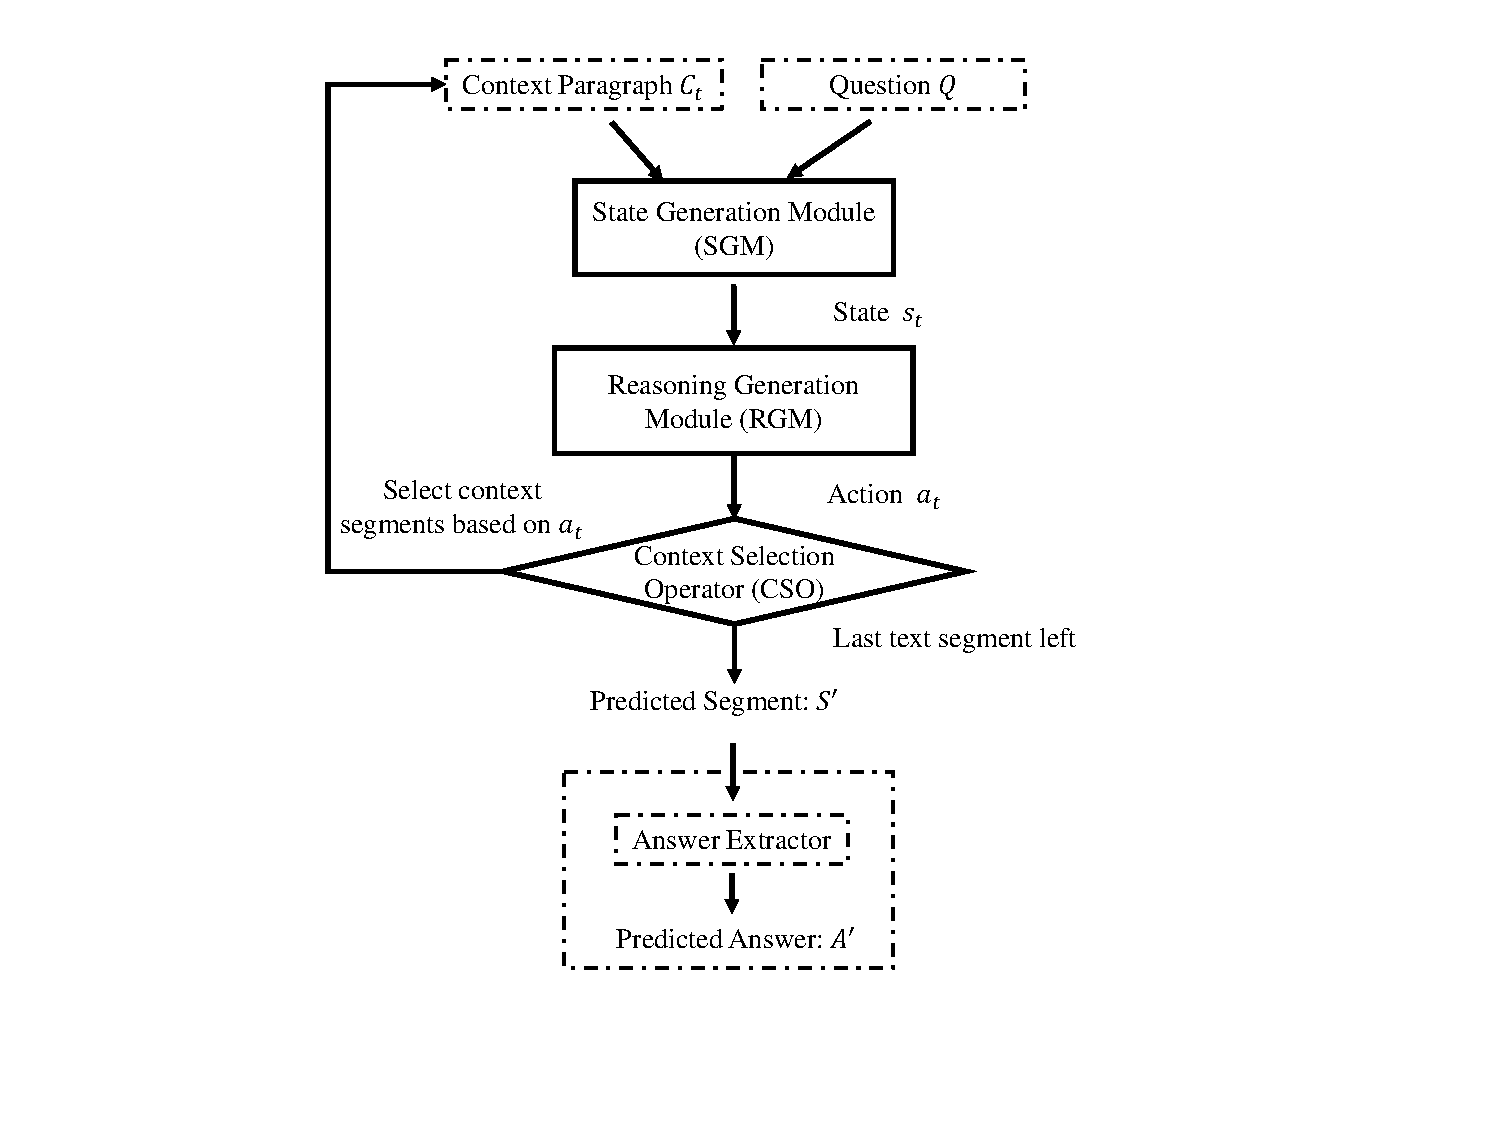
\includegraphics[width=0.9\linewidth]{fig/fig1.pdf}
 \caption{System Diagram}
 \label{fig:systemDiagram}
\end{minipage}
\vspace{-2ex}
\end{figure}
%[Yu] \kechen{basic idea of RL and insight of using RL, multi step decision is naturally modeled by MDP}
% \subsection{Model Component Overview}
\label{sec2description}
The goal of our system is to mimic human reading behavior to extract a segment that
contains the answer. The mechanic in reducing the text context is analogous to binary search: Let $D=(D^1,D^2,...,D^k)$ be a list of discourse markers that appears in a context paragraph $C$. These discourse markers, working as the candidate partition points, divide the context into a list of segments $S=(S^1,S^2,...,S^{k+1})$. Then the context can be represented by a mixture of discourse markers and segments, $C=(S^1, D^1, S^2, D^2,...,D^k, S^{k+1})$. To identify the correct segment $S^*$ from $S$, our model at time-step $t$ works as follows:\\
(a) SGM encodes the context $C_t$ and question $Q$ into a vector representation, \emph{i.e.} the state $s_t$.\\
(b) RGM takes the state $s_t$ as its input, and predicts the partition point $D^{p(s_t)}_t$ (${p(s_t)}$ is the index selected at \emph{t}) and the reading focus $f_t \in \{left, right\}$. An action is defined as $a_t=(D^{p(s_t)}_t,f_t)$. \\
(c) CSO divides $C_t$ into two parts from $D^{p(s_t)}_t$: $C^1_t=(S^1, D^1,...,D^{p(s_t)-1}, S^{p(s_t)})$ and $C^2_t=(S^{p(s_t)+1}, D^{p(s_t)+1},...,D^k, S^{k+1})$, and keeps $C_{t+1} \leftarrow C_{t}^{1}$ if $f_t$ is left or $C_{t+1} \leftarrow C_{t}^{2}$ if $f_t$ is right. \\
The iterations stop when the output only contains a single text segment enclosed by two neighbor discourse markers. Intermediate output $D^{p(s_t)}_t$ at each time-step constitutes a reasoning path $(D^{p(1)}_1,...,D^{p(s_t)}_t)$. We note that during the prediction procedure the context $C_t$ changes, while the question $Q$ not (see Algorithm~\ref{alg:train_beam}).

% \emph{Remarks:}
It is possible to add an answer extractor following the text segment $S'$ for a final answer (dashed in Figure \ref{fig:systemDiagram}). Since this is not our paper's focus and many existing works have been done achieve decent performance \cite{DBLP:conf/ijcai/HuPHQW018}, so this module is not discussed in this paper. %\cite{DBLP:conf/acl/WangYWCZ17,DBLP:journals/corr/abs-1804-09541,DBLP:conf/ijcai/HuPHQW018}. Since this is not our paper's focus, we do not discuss it here.\\


%Since our paper's focus is not on answer extraction, and many existing works have been done achieve decent performance \cite{DBLP:conf/acl/WangYWCZ17,DBLP:journals/corr/abs-1804-09541,DBLP:conf/ijcai/HuPHQW018}, so this module is not discussed in this paper.



\begin{algorithm}
\fontsize{9}{10}\selectfont
  \SetKwInOut{Input}{Input}
  \SetKwInOut{Output}{Output}

 % \underline{function Euclid} $(a,b)$\;
  \Input{$C$: context, $Q$: question}
  \Output{Answer segment: a single text segment enclosed by two neighbor discourse markers}
  $t = 0$\\
  $C_0 \leftarrow C$\\
  % Initialize model parameters\\
  \While {$C_t$ contains more than one text segment}{
    %SGM encodes the context $C_t$ and question $Q$ into a vector representation $s_t$.\\
    $s_t = SGM(C_t, Q)$ // generate state\\
    $D^{p(s_t)}_t,f_t= RGM(s_t)$ // generate action\\ 
   % $a_t=(D^{p(s_t)}_t,f_t)$ // an action consists of partition point $D^{p(s_t)}$ and reading focus $f_t$\\
    $C^1_t, C^2_t = CSO(C_t, D^{p(s_t)}_t)$\\
    \uIf{$f_t==left$}{
    //$C^1_t=(S^1, D^1,...,D^{p(s_t)-1}, S^{p(s_t)})$\\
        $C_{t+1} \leftarrow C_{t}^{1}$ 
    }\Else{
    //$C^2_t=(S^{p(s_t)+1}, D^{p(s_t)+1},...,D^k, S^{k+1})$\\
        $C_{t+1} \leftarrow C_{t}^{2}$ 
    }
    $t = t + 1$
  }
  $S^* \leftarrow C_t$\\
  \Return{$S^*$}
  \caption{Identifying the correct answer segment from the context}
	  \vspace{-1ex}
  \label{alg:train_beam}
\end{algorithm}
\subsection{Deep Reinforcement Learning}\label{sec2intuition}
%As described in the introduction, in order to build a "smart" machine comprehension system by imitating a human-like reasoning process, we leverage a deep reinforcement learning (DRL) based structure to infer the reasoning steps guided by the discourse markers and/or the target words. There are two main reasons to choose DRL as our fundamental model structure:\\

We leverage a deep reinforcement learning (DRL) based structure to implement the system introduced in the above section. 
For every given context-question pair, the dataset provides an answer. Although this answer can be used to evaluate the final output of any reasoning path, there is no ground truth to evaluate the performance of each intermediate reasoning step $D^{p(s_t)}_t$. There are usually several different reasoning paths leading to the correct answer segment, based on different sequences of selecting discourse markers; thus the  task of searching for the best path fits well into the reinforcement learning, as these actions can reasonably imitate the human actions.
% , which makes our model more interpretable.
% It enables a flexible number of action steps to gradually search for the correct answer instead of generating the answer from end-to-end.
%There are also many possible reasoning paths which can lead to the same correct answer. In order to search such a reasoning path, %, just like searching for one possible route in a maze, DRL based approaches are very suitable. 

%2.  \kechen{merge 1 and 2? introduce reasoning path?}

A typical reinforcement learning structure contains four main elements: the state ($s_t$), the action ($a_t$), the reward ($r_t$), and the policy ($\pi$). In general, by taking an action $a_t$, a RL agent can move from its current state $s_t$ to another state $s_{t+1}$ and receive a reward $r_t$. The final target of a RL model is to learn an optimal policy $\pi$ such that the system can maximize the expected total reward $R_t=\mathop{\mathbb{E}}_\pi[\sum_{t=0}^{T}\gamma^t r_t]$ obtained at each state $s_t$, where $s_T$ is the final state. Specifically in our problem, at each time-step $t$ our model is in state $s_t$ containing the information of the current context $C_t$ and the question $Q$; it takes action $a_t$ choosing the appropriate discourse marker and the direction (reading focus) in order
to maximize the expected reward $R_t$. 
%*This expected reward can be further interpreted as the probability of finding the final correct answer by choosing this discourse marker and its reading direction.

%\cheng{unclear}
% \section{Model Design}
\label{sec:model}

%Figure XXX shows a general structure of our model. It contains three major components: a state generation module (SGM), a DRL reasoning module (DRLM) and an action selection module (ASM). Before discussing the details in next section, we briefly review the terms used in a (conventional) reinforcement learning model.

%As in Markov Decision Process (MDP), a conventional reinforcement learning structure contains four main elements: the states, the actions, the rewards and the policy. In general, by taking an action $a_t$, an agent can move from the current state $s_t$ at time $t$ to another state $s_{t+1}$ at time $t + 1$. The agent receives reward $r_t$ at each state $s_t$. A discounted reward $R_t$ \cheng{should be $R_{t_0}$?} is then calculated as
%\begin{equation}
%R_t=\sum_{t=t_0}^\infty \gamma^{t-t_0}r_t$
%\end{equation}
%where $\gamma\in[0,1]$ is the discount factor, and $t_0$ indicates the starting time step.
%The target of a reinforcement learning process is to learn a final policy $\pi$ containing an action-state mapping such that the maximum expected rewards can be obtained through learning, \emph{i.e.}
%\begin{equation}
%V^\pi(s_t,a_t)=\max_{\pi}\mathbf{E}[R_t|a_t,s_t,\pi].
%\label{eq:optL}
%\end{equation}
%where $V^\pi(\cdot)$ is the optimal action-value function.
%Specifically in our system, we use the information from the context document and question to generate the RL states using the state generation module (SGM), and use the connectives/discourse markers to design our actions in the action selection model (ASM), and an actor-critic based DRL model to construct the DRL reasoning module (DRLM). In section \ref{sec:model}, the designs of states, actions, rewards and policies in the three submodules of our system will be given in detail. A actic-critic based DRL training algorithm is also explained.

% Following the system structure and the reinforcement learning terms defined in last section, in this section, we would like to describe the designs of these components in our deep reasoning model in detail.
% 
%\cheng{We need a high level description of how the algorithm works, before we turn that intuition in to math. Something like a binary search -- choose a discourse marker, move left and right, and so on. We need to give readers a big picture first. }


\begin{figure}\centering
\begin{minipage}{.45\textwidth}
 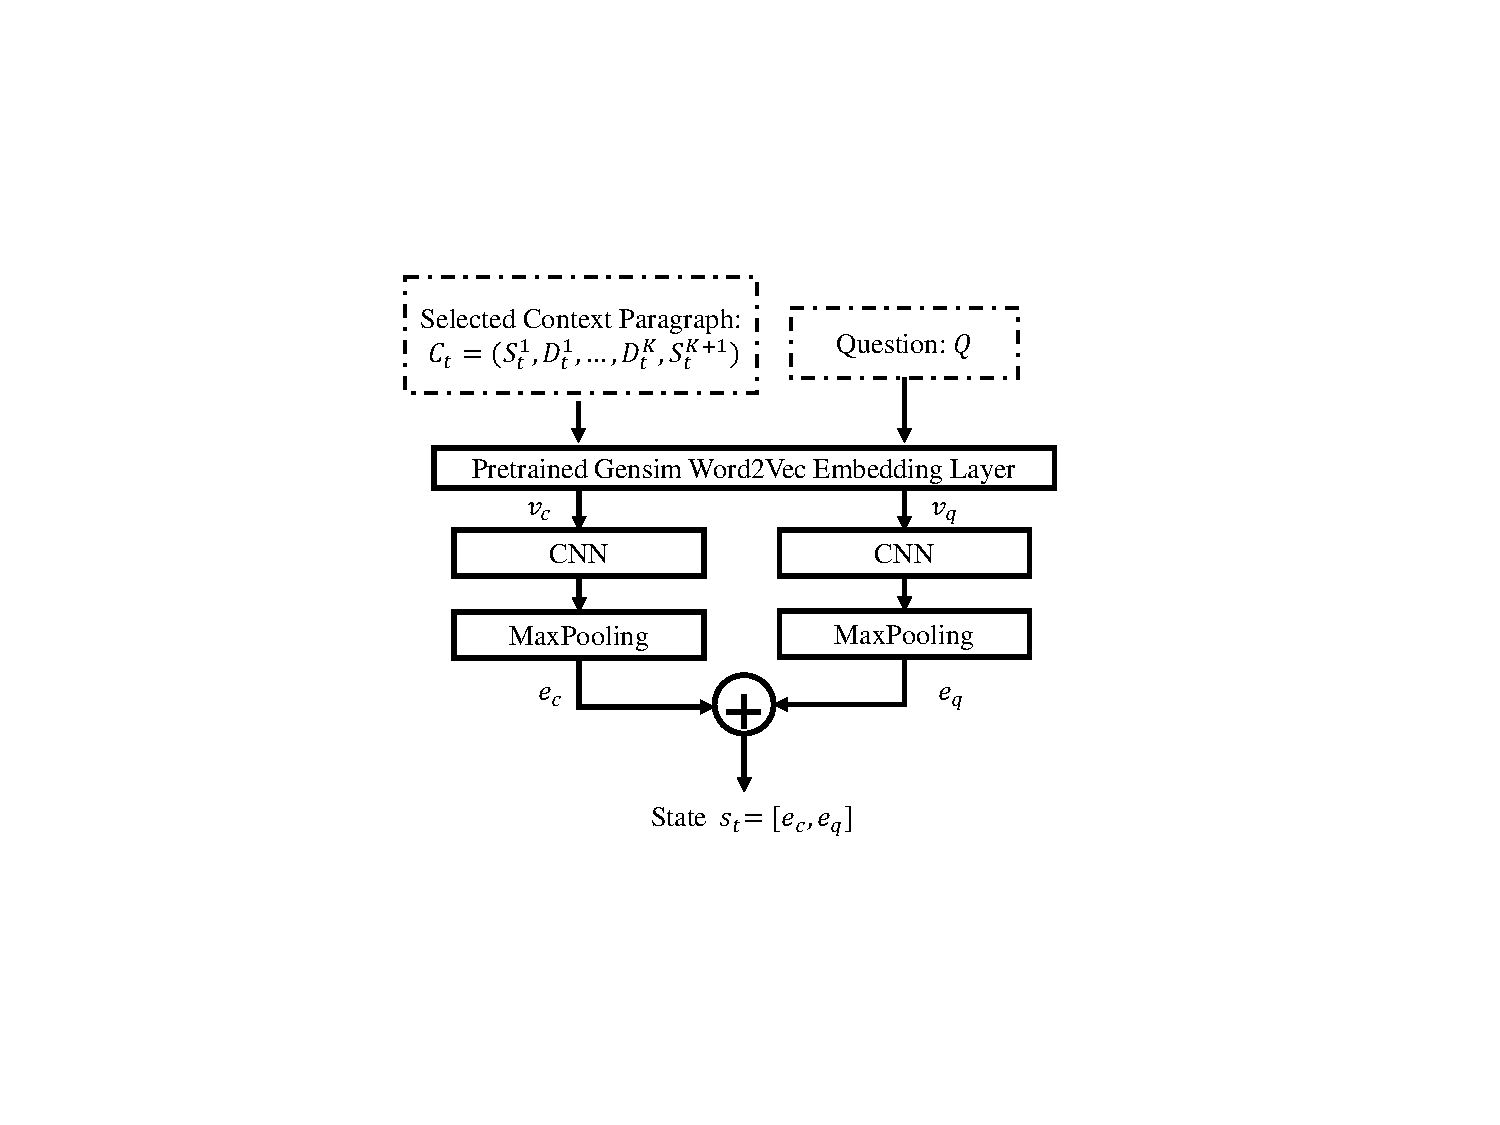
\includegraphics[width=0.9\linewidth]{fig/fig1_2.pdf}
 \caption{SGM Diagram}
 \label{fig:sgmDiagram}
\end{minipage}
\vspace{-2ex}
\end{figure}

\subsection{States, Actions, Rewards}\label{sec:design}
%\cheng{Before talking about states, we should define what is a time step, and what changes from step to step. Question does not change. The segment that we are looking at changes? Because the concept of step is introduced by us, we cannot assume that the readers know it. It's not like in chess where steps are a well known notion}

\textbf{Design of State:} As our system's input, a state contains the information from both the context and the question (as shown in Figure \ref{fig:sgmDiagram}). %we designed state generation model (SGM) to generate their embeddings in order to construct the defined states. First, we train a preliminary word embedding dictionary using the gensim word2vec on a given dataset. By using these pre-trained word embeddings, 
We feed the context paragraph and the question separately into our state generation module (SGM), which contains an embedding layer and a convolutional layer followed by a max-pooling layer. The obtained embedding of the context paragraph is concatenated with that of the given question, in order to form a state as the input to RGM. The embedding layer is pre-trained using our dataset; the CNN and max-pooling layers are trained and updated together with our RL model. %, whose outputs are the actions to be defined in next section. Using this two-step approach, we can both leverage the fixed word-level information from our corpus and learn-able embedding information guided by the expected rewards obtained in DRL. %\kechen{add why we don't use coattention and intuition of choosing CNN}
%\subsection{Design of Actions}\label{design_action}
 %As defined in section XXX, t
 
 \textbf{Design of Actions:} The actions determine the reading focus at next time-step $t+1$. 
 % The design of actions is supposed to be close to one type of our human reasoning behaviors: using discourse markers and question topic to guide reading.
 Two different set of action designs are introduced as follows:
 
{\bf{ \underline{Action Set $1$:}}}
The first set of actions is designed only using the discourse markers, such that for each action, either context paragraph before or after a marker is chosen to be focused. An action is supposed to contain two pieces of information: (a) the word marker to be selected, and (b) the focus of reading from the selected marker, \emph{i.e. left} or \emph{right}. The action space is defined as $\lbrace\alpha_{1}^{left},\alpha_{1}^{right}, \cdots,\alpha_{k}^{left},\alpha_{k}^{right}\rbrace$, where $k$ discourse markers are selected from our discourse marker lexicon. The entire action space dimension is $\mathbb{R}^{2\times k}$ by considering the left and right directions. %After choosing an action, for example $\alpha_{i}^{left}$, the system will focus on the context \emph{left} to the discourse marker $d_{i}$, and vice versa for $\alpha_{i}^{right}$.

%\vspace{-1.0mm}
%\begin{itemize}[itemsep=0.1mm]
%\item The word marker to be selected.
%\item The focus of reading from the selected marker, \emph{i.e.} left or right.
%\vspace{-1.0mm}
%\end{itemize}
%In our model, we use the discourse marker, which is a main type of connectives, as the word markers described before. 

%which divide a document into multiple sentences/phrase segments. As in XXX, a human reader would like to use a word marker for reasoning in a machine reading task, %\cheng{I am not sure there is how humans read. I am not sure that the reviewers will buy this argument. Is there any behavior or psychological study that shows humans search for answers this way?} 
%Assuming that our system wants to imitate this learning process, our system's 
%Inspired by the work in XXX, in our model, we use the discourse markers, which is a main type of connectives, as the word markers for the model to select in this type of action design. 
%Furthermore, we also use the combination of discourse markers and target word(s) to define our action as shown in the second type of action design. \cheng{This is repeated in earlier sections}

%Also, in order to limit the action space size, we only select top $k$ discourse markers from XXX ranked by their frequencies in our datasets. By considering the searching directions from the selected discourse marker(s), the action space size is $2\times k$, which is the double of number of discourse markers selected. 
%A graphical illustration is as shown in Figure XXX:

%The action space includes $2\times k$ actions. At each time step $t$, the system selects one of them as the output of our DRL model. Specifically in our case, the DRL model will generate an action vector with a size of $2\times k$, where one of numbers in the vector is 1, and all the others are equal to 0s\kechen{why is that?}.


 {\bf{\underline{Action Set $2$:}}} The second set of actions leverages the information from both the discourse markers and the question topic. In our work, a target word is extracted from the question to capture question topic information. %By adding one more piece of information indicating the user's intention, 
 We expect that this action type can give better reasoning performance by associating the discourse information in context with the topic in question. The action space is defined as $\lbrace\alpha_{1}^{target},\alpha_{1}^{target\_{rev}}, \cdots,\alpha_{k}^{target},\alpha_{k}^{target\_{rev}}\rbrace$. After selecting an action $\alpha_i^{target}$, the system will focus on the text towards the direction to the target word from the discourse marker $d_i$ by ignoring the the text in the reverse direction; otherwise if action $\alpha_i^{target\_{rev}}$ is selected, the system will focus the text in the reverse direction to the target word from the discourse marker $d_i$, by ignoring the text in the same direction to the target word. For example, $\alpha_{ind(``until")}^{target\_{rev}}$ is selected in reasoning step 1 in Figure \ref{fig:qa_example} with the target word ``reheating", where $ind(*)$ returns the index of a word. It is worth noticing that if the same marker appears twice in a  selected context, the marker which is closer to the target word is picked.
 %\kechen{kechen add some intuition and entropy result}
%The action space is as shown in figure XXX.

 %To help better understand these action definitions, we also use an example to explain each action operation as in Figure XXX. \kechen{kechen add example}
 
 %\subsection{Design of Rewards}
\textbf{Design of Rewards:} 
% Another important element in reinforcement learning is the reward $r_t$, which can greatly affect the performance and robustness of a DRL model. In our system,
The reward $r_t$ is defined as whether the predicted segment $S'$ is the same as ground truth $S^*$ or not.
If it is, the reward is 1, otherwise it is 0. It is also worth noticing that the reward is only assigned to the final state, \emph{i.e.} no further action(s) to be performed for that context paragraph. The reward at other time-steps is 0.

%In our scenario, the ground truth $A^*$ is the correct answer given a context and a question. 

\subsection{Actor-Critic Algorithm}
%\kechen{2.6 is incomplete? In particular, I need more information to understand the objective functions in equation 1.}
 % In this work, we use the actor-critic based algorithm  to build our DRL model. %Unlike the value based DRL approach like DQN \cite{mnih2015human} or policy based approach like policy gradient \cite{sutton2000policy}, an actor-critic based model has a better performance on continuous state space in terms of convergence and stability.
 % Due to the space limitation and the focus of this paper, we will only describe the actor-critic method briefly.
%\subsubsection{Training}

In an Actor-Critic based DRL algorithm, two separate neural networks are built to model the actor and critic. The actor updates the policy parameters $\theta$ for $\pi_\theta(a_t|s_t)$, while the critic predicts an expected reward at that state to assist the policy update. %The actor model performs like a policy gradient approach \cite{sutton2000policy} by taking state $s_t$ as its input and generating action probabilities based on the policy: $\pi_\theta(a_t|s_t)$. Comparatively, the critic model applies a value based algorithm, like $DQN$ \cite{mnih2015human}. 
At each training iteration, by performing the action $a_t$ generated by actor, the system transits to a new state $s_{t+1}$ from its current state $s_t$, and then the critic  can generate two values (\emph{i.e.} expect rewards) $v_t$ and $v_{t+1}$ by taking $s_t$ and $s_{t+1}$ as inputs. There are two separate loss functions, training the actor and the critic models:
\begin{equation}
%\vspace{-0.5ex}
\begin{split}
\mathcal{L}_{actor}&=-\log \pi_{\theta} (a_t|s_t)(r_t+\gamma v_{t+1}-v_{t})\\
\mathcal{L}_{critic}&=(r_t+\gamma v_{t+1}-v_{t})^2
\label{rlloss}
\end{split}
\end{equation}
where $\gamma$ is a discount factor in our DRL model. From the loss function, we can see that the actor model aims to maximize the expected rewards to be obtained, and the critic model minimizes the temporal difference error during the stochastic learning process. Compared to the commonly used policy-gradient RL algorithm, an actor-critic based model has a better performance in terms of convergence and stability. During inference, our model reads in a sample containing the full context paragraph $C_0$ and question $Q$. At each time step $t$, the model generates an action which leads to a new context paragraph $C_{t+1}\subset C_t$. This inference process stops when there is no discourse marker contained in the current context paragraph, which is also the final predicted segment $S^{\prime}$ as in Figure \ref{fig:systemDiagram}. During training and inference, if the selected discourse marker does not appear in the context, the model will do the selection again.
%In this definition, we can find that the actor model aims to maximize the expected rewards to be obtained, and the critic model minimizes the temporal difference error during the stochastic learning process. %\kechen{during prediction, we use greedy search to ... add the connection to our setup}
%\kechen{we keep sampling until the sampled action is available.}
%\subsection{Prediction}
 %The model's accuracy is evaluated by the percentage of prediction segments containing the ground truth answer $A^*$.
%\cheng{I think we need to add a subsection to talk about how to make predictions; otherwise the model is incomplete}
\section{Experiments and Data}
% \subsection{Data Description}
%\kechen{highlight importance of using discourse marker, one sentence may contain more than one answer candidate, which makes NN model hard to distinguish.}
\textbf{Discourse Markers Lexicon.}
%In Rhetorical Structure Theory (RST) discourse framework \cite{mann1988rhetorical}, the text is segmented into a sequence of non-overlapping fragments called elementary discourse units (EDUs), and discourse relations connect neighboring units. Both EDUs and discourse relations, encoding the useful information about syntactic and semantic pragmatic properties, play important roles in understanding the context structure and extracting answers given a query \cite{DBLP:conf/clin/Bosma04,bosma2005extending,DBLP:journals/tal/VerberneBCO06,DBLP:conf/acl/JansenSC14,DBLP:conf/acl/NarasimhanB15}. Because discourse analysis is notoriously difficult, existing work seeks to utilize discourse markers to determine discourse relations, and thus identify the EDUs \cite{adequacyusing,sporleder2007exploiting,}. In this work, discourse markers guide the model to distinguish the answer-relevant text segments or EDUs from the context. \kechen{rewrite}
To build a lexicon of English discourse markers, we collect connectives from Penn Discourse Treebank 2.0 (PDTB2.0) \cite{DBLP:conf/lrec/PrasadDLMRJW08} and \cite{marcu1998rhetorical}'s list of cue phrases. Inspired by a recent work \cite{DBLP:conf/sigdial/DasSBS18}, we add to our list additional words from RST Signalling Corpus \cite{das2014rst}, DiMLex-Eng corpus \cite{DBLP:conf/sigdial/DasSBS18}, and \cite{DBLP:journals/ijsc/BiranR11}'s relational indicators. After filtering out discourse markers with low frequencies in our corpora, we get a list of 207 discourse markers. Table \ref{tab:discourse_markers} shows sample discourse markers with their senses\footnote{Although in most of the cases the discourse markers can separate arguments with different meanings, some of the discourse markers such as ``although'' and ``if'' can precede both arguments, \textit{e.g.``although her friends like ice cream, she prefers yogurt''.} To deal with these cases, we add ``,'' into our sets of discourse markers to help.}. 
\begin{table}[t]
\centering
{
	\fontsize{8}{9}\selectfont
    %\setlength{\baselineskip}{0pt}
    \setlength{\tabcolsep}{1.0mm}
    \renewcommand{\arraystretch}{1.1}
	%\hspace{4mm}
	\begin{tabular}{|c|c|}
 	\hline
  	\textbf{Sense} & \textbf{Sample discourse markers} \\
  	\hline
 	concession& although, though, but, if, however   \\
    \hline
 	conjunction& and, then, or, while, also \\
 	\hline
 	cause & because, because of, as, since, as a result  \\
 	\hline
 	asynchronous& before, when, previously, until,after \\
 	\hline
 	restatement& rather, in turn, particularly, in particular, indeed   \\
 \hline
\end{tabular}
}
\caption{\fontsize{10}{12}\selectfont Sample discourse markers and their senses.}
\label{tab:discourse_markers}
\vspace{-2ex}
\end{table}

\textbf{RC Corpora.}
There are many QA datasets (\textit{e.g.} SQuAD \cite{DBLP:conf/emnlp/RajpurkarZLL16,DBLP:conf/acl/RajpurkarJL18} and CNN/Daily
News \cite{DBLP:conf/nips/HermannKGEKSB15}) available for reading comprehension tasks. Most of the documents in these datasets, however, don't contain dense discourse markers, thus they are not suitable to test our model's performance. 
%Although deep neural networks perform well on these datasets, they fail to explain long path reasoning. 
To demonstrate our model, we focus on Question-Answer meaning representations datasets \cite{DBLP:conf/naacl/MichaelSHDZ18}: the QAMR corpus and the PTB corpus. Both of them contain relative short-document context but with complex logic reasoning steps. Specifically, the Wall Street Journal (WSJ) documents in PTB corpus are widely used in discourse studies. We restrict our discussion to shorter documents by filtering out documents without discourse markers and those with more than 10 discourse markers; this is because an excessive number of discourse markers in long document tends to give redundant reasoning steps. Binary searching by discourse markers in such long documents is not necessarily how human read and interpret long expositions, so our method is less applicable.
% , which is also kind of different from a normal human's reading behavior. Removing such samples can also helps us reduce the total training time.
%This study uses two corpora from Question-Answer Meaning Representations datasets \cite{DBLP:conf/naacl/MichaelSHDZ18}: the QAMR corpus and the PTB corpus. They contain QA pairs extracted from Wikipedia and Penn Treebank \cite{DBLP:journals/coling/MarcusSM94}.
%The QAMR corpus consists of 69,320 QA pairs for 4,238 context paragraphs extracted from Wikipedia, and the PTB corpus consists of 27,082 QA pairs for 253 context paragraphs extracted from Penn Treebank \cite{DBLP:journals/coling/MarcusSM94}.
There is one target word in each question representing the question topic associated with each QA pair. %We treat a QA pair and its context paragraph as one data sample. 
When the answer spreads across two text segments, we treat the discourse segment containing more than 50\% answer tokens as the answer segment.
%We assume that the answer cannot spread across two text segments, and remove those counter-cases (Only 8\% QA pairs are counter-cases.), so each context only contains one segment 
% enclosed by discourse markers containing the ground truth answer. 
After pre-processing, 5\% QA pairs are filtered out from the original dataset, and the two corpora in our experiments are referred as \textsc{QAMR-SUBSET} and \textsc{PTB-SUBSET}.
% These two datasets are suitable to our reading comprehension experiments and transferable experiments, as they contain a variety of questions that are from different sources.


\textbf{Experimental Setup.}
We implement our deep reasoning model (DRM) using \textsc{tensorflow-1.4.0} and \textsc{Keras-2.0.8}. To implement CNNs, we use rectified linear units (relu) as activation functions and 300 convolutional filters with windows size of 2. We train the model with Adam optimizer with start learning rate $0.001$. We adopt \emph{accuracy} as our main evaluation metric, which measures how many selected text spans contain the answer out of all. The following  methods are compared:\\
% \begin{itemize}
% \vspace{-1mm}
% \setlength\itemsep{-0.8mm}
$\bullet$ \textbf{DRM-type 1} and \textbf{DRM-type 2} Our deep reasoning models with type 1 /type 2 action. \\
% $\bullet$  \textbf{DRM-type 2} Our deep reasoning model with type 2 action, as described in Section \ref{sec:design}. \\
$\bullet$  \textbf{DRM-type 2 w/ human} We consider a variant of our deep reasoning model with human in the loop, in order to demonstrate that our model has the ability to interact with humans. At each decision step, if the algorithm's confidence in its best action is lower than a pre-specified threshold $T_r=0.6$, the algorithm asks a human to pick an action from the $2\times k$ actions. We assume that humans always make the right decision w.r.t. the ground truth.  \\
$\bullet$  \textbf{DRM-noRL} We test our model structure with multi-class classification loss. Each segment is assigned a score, and the segment with the highest score is predicted. \\
 $\bullet$  \textbf{Gradient Boosting}. 
 % A  binary classifier to evaluate different (question, context segment) pairs and select the segment with the highest prediction score. corollary
% Bag-of-words features are first extracted separately from both the question and the segment and then concatenated. We choose Gradient Boosting due to its effectiveness in modeling feature interactions;
Two variants of Gradient Boosting are tested, one trained with binary cross entropy loss, and the other with ranking loss. In addition to bag-of-words features, for fairness we introduce four new discourse features: left and right discourse markers, the position of the target word, the first word of the question.\\
$\bullet$  \textbf{BM25} We use BM25~\cite{DBLP:journals/ftir/RobertsonZ09} as a bag-of-words retrieval function to rank segments based on the question terms. \\
%$\bullet$  \textbf{Chunked BoW Model}~\cite{DBLP:conf/acl/ChoiHUPLB17}. This is similar to the Gradient Boosting-binary model, except that the binary classifier employed is a neural network with fully connected layers. \\
$\bullet$  \textbf{Coarse-to-Fine Answer Selector}~\cite{DBLP:conf/acl/ChoiHUPLB17} concatenates the context and the question, and run a neural network on it to select the relevant text span. We adopt their Chunked BoW setup.\\
$\bullet$  \textbf{RaSoR}~\cite{DBLP:journals/corr/LeeKP016} builds a deep neural network model to select a span of text as the answer. Each candidate span is fixed-length representated using BiLSTM and neural co-attention. 
% \end{itemize}

\subsection{Experimental Results}
%0. RL learning curve\\




We report the overall segment prediction accuracy on the datasets and the accuracy on each question type (Table~\ref{tab:main}). On both QAMR dataset and PTB dataset, DRM-type 2 with human in the loop achieves the highest accuracy. Being able to interact with humans is an advantage of our approach; 
% Humans can understand the decision process of the algorithm and can intervene if necessary. By contrast, 
none of the competitor approaches can do this, either because their decision process is a single-step process or because their decision process is not interpretable. In our experiment, 65\% QA pairs (less than the threshold) get help from human at one reasoning step, and their performance increases 0.15. It is also very interesting to learn that the remaining 35\% data points with high confidence reasoning learned by our model perform 0.06 better than the average performance. To further understand whether the improvement comes from human's selection or from our model's judgement, we allow the model to randomly select 65\% of the QA pairs, and for each pair, to interact with human once without considering their confidence. The results show that such random selection procedure doesn't make any difference on performance. Even without human's help, our DRM-type 2 model still achieves better performance than all other methods. As expected, DRM-type 2 model performs better than DRM-type 1 model, since type 2 actions leverage more information. 
%Looking at how the algorithm performs as the number of reasoning steps increases, the prediction accuracy increases slightly as the reasoning gets longer: the accuracy for 1-step, 2-step, 3-step and 4-step reasoning is 0.700,0.700,0.705 and 0.727.

Among the baseline methods, Gradient Boosting trained on both bag-of-words + discourse features works best. These models perform much worse if trained only on bag-of-words features. This shows that the structure/order information captured by discourse features is essential, which Neural network doesn't do. 
% The classical BM25 works well on questions that start with ``whose" but terribly on questions that start with ``why". 
Since BM25 solely relies on similarity between the question and the segment, it only works well when the the question and the correct segment have many overlapping words, as in the case of ``whose" questions, but not ``why" questions.

We also study whether the learned reasoning model is transferable by training DRM on the QAMR dataset but test the learned model on PTB dataset. Results in Table~\ref{tab:main} show that this model generalizes well on PTB dataset -- its performance is very close to the DRM model trained on PTB directly. We also observe that the RaSoR model achieves a very good performance. We think this is because training a deep neural network model benefits from the larger number of training samples in QAMR dataset. 


\subsection{Comparison with QA Methods}
In this section, we compare our model with several other benchmark QA models on the QAMR and PTB datasets. The results are shown in Table~\ref{tab:nnresults}. 
\begin{table}[h]
	\centering
	\resizebox{0.8\columnwidth}{!}{%resize the table
\begin{tabular}{|l|c|c|}
  \hline
  \textsc{Model} & \textsc{QAMR} & \textsc{PTB}   \\
  \hline
  MemNets & .476 & .423 \\
  GA-Reader (fix $L(w)$) & .610 & .532 \\
  QANet & .703 & .602   \\
  Mnemonic Reader & .700 & .595 \\
  DRM-type 2 & .702 & .599   \\
  \hline
\end{tabular}
}
\caption{\fontsize{10}{12}\selectfont  Our model vs. popular QA models.}\label{tab:nnresults}
  \vspace{-2ex}
\end{table}
Most of these approaches are originally designed to extract the exact answer(s) from the context. In order to modify these models' outputs as a segment, we change the training target from the exact answer to an answer segment. We observe that QANet gives the best accuracy in terms of selecting the correct text span containing the answer. 
% All these methods except QANet can be considered as multi-step reasoning models, and our model gives the best performance among all these models.
% 1. discourse is better than no discourse in Gradient Boosting and Gradient Boostingrank
% 2. bm25 model similarity, perform not very well e.g. 'The victory comes (after) a few days (because)blabla' What comes a few days after?
% 3. bow and cnn can't explicitly model discourse info, so perform not very well
% 4. compare two setups? binary classifier vs. pairwise ranking
% 3. drmtype2 perform better than drmtype1 as we expected
% 4. introduce how human-in-the-loop work
% 5. 
% 6. compare drm-transfer and drm-ptb: why better than ptb why because ptd does not contain many why question.


%Because the deep reasoning model appear to capture high-level information about context structures, we hypothesize that the models should perform very well even when training on data from different domains. http://www.aclweb.org/anthology/P14-1092


\begin{table*}[t]
\centering
{
	\fontsize{9}{9}\selectfont
  %\setlength{\baselineskip}{0pt}
  \setlength{\tabcolsep}{1.0mm}
  \renewcommand{\arraystretch}{1.1}
	%\hspace{4mm}
	\begin{tabular}{|p{1.8cm}|p{2.5cm}|p{2.5cm}|p{2.5cm}|p{5.8cm}|}
 	\hline
 	\textbf{Question genre}  & \textbf{Same side}& \textbf{Opposite sides}& \textbf{Context-dependent (side)} &  \textbf{Example QA pairs} \\
 	\hline
 	when \newline what year \newline how long 
 	& \textbf{step 1}: already, again, still, following \newline\textbf{step 2}: while, yet & \textbf{step 1}: as soon as, at that \newline\newline \textbf{step 2}: then, further, originally
 	&\textbf{step 1}: previously, until, back, after, soon, during \newline \textbf{step 2}: since, second, next, when, as well, because, who 
	&  \textbf{Context: }28 \textit{\textcolor{blue}{skiers}} earned DNFs \textit{\textcolor{red}{during}} \underline{the first run}, \textit{\textcolor{red}{and}} nine earned DNFs \textit{\textcolor{red}{during}} their second runs.
  \newline \textbf{Question: }When did \textit{\textcolor{blue}{skiers}} earn DNFs? 
  \newline \textbf{Learned Reasoning: } during-right, and-left\\ 
	\hline
  why \newline what caused 
 &\textbf{step 1}: in order to, because, due to,  since \newline\textbf{step 2}: as, but &\textbf{step 1}: at that, previously, though, if, since \newline \textbf{step 2}: second, for, to, or, that, not, and & \textbf{step 1}: well, following, initially  \newline\newline\textbf{step 2}: which, even,certainly  
  & \textbf{Context: }Given its initial condition, prediction of its final condition is possible, causally \textit{\textcolor{red}{but}} only probabilistically, \textit{\textcolor{red}{because}} the Schrödinger equation is deterministic for wave function evolution, \textit{\textcolor{red}{but}} \underline{the wave function describes the system only} \underline{\textit{\textcolor{blue}{probabilistically}}}.
  \newline \textbf{Question: }Why is the prediction \textit{\textcolor{blue}{probabilistic}}?
  \newline \textbf{Learned Reasoning: }because-right, but-right\\ 
	\hline	
	who+past tense 

	& \textbf{step 1}: rather, thus, including \newline\newline\textbf{step 2}: nor, who, initially &\textbf{step 1}: earlier, definitely, previously \newline\newline\textbf{step 2}: particularly, seemingly
		&\textbf{step 1}: ultimately, since, when, later, while, finally \newline \textbf{step 2}:  again, last, and , after, next, 
	& \textbf{Context: }\underline{Hatch had} \textit{\textcolor{red}{previously}} \textit{\textcolor{blue}{survived}} a separate crash in 2003, \textit{\textcolor{red}{that}} killed his mother, brother \textit{\textcolor{red}{and}} sister.
  \newline \textbf{Question: }Who \textit{\textcolor{blue}{survived}}?\newline \textbf{Learned Reasoning: }previously-left\\ 
	\hline
  where 
 
  
	 &\textbf{step 1}: following, to explain, while \newline\newline\textbf{step 2}: possibly, initially, finally, hence &\textbf{step 1}: to, before, back, in that, eventually \newline\textbf{step 2}: like, or, as & \textbf{step 1}: in which, then, second, next \newline\newline \textbf{step 2}: too, yet, second, including, after, next
  & \textbf{Context: }\textit{\textcolor{red}{Once}} the proposed \textit{\textcolor{blue}{amendment}} has passed those hurdles, \textit{\textcolor{red}{then}} the amendment goes \textit{\textcolor{red}{to}} \underline{Indiana voters} \textit{\textcolor{red}{who}} vote yea or nay on the amendment. 
  \newline \textbf{Question: }Where does the \textit{\textcolor{blue}{amendment}} go?
  \newline \textbf{Learned Reasoning: }to-right, who-left\\ 
 \hline
\end{tabular}
}
\caption{\fontsize{9}{12}\selectfont Top discourse markers are associated with question genres, and focus direction is learned in \textsc{QAMR} dataset. We show four different question genres: time, reason, person, and location.}
\label{tab:disc_phrase}
\vspace{-3ex}
\end{table*}

Our method has an obvious advantage over the others: unlike the multi-step models where the number of steps need to be predefined, our model is capable of using a dynamic number of reasoning steps to resolve different QA pairs. Another very important difference is that the existing models achieve multi-step by updating the internal vector representations, which is not interpretable, while our model directly prunes the context for an interpretable reasoning process.

\subsection{Experiment on SQuAD}

\begin{figure}
 \centering
 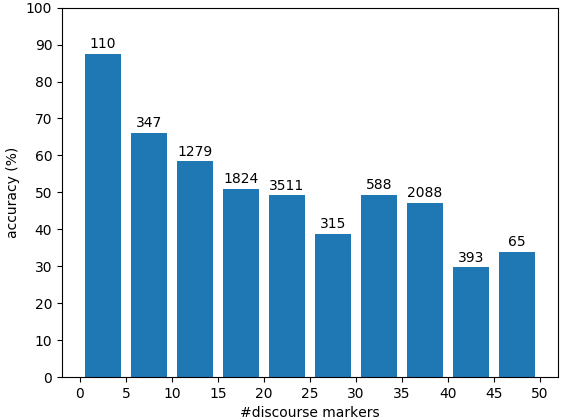
\includegraphics[width=0.9\linewidth]{fig/squad.png}
 \caption{\kechen{Accuracy on each discourse marker interval of SQuAD dataset, which contains 10,570 documents. We show the number of documents in each interval on top of each bar.}}
 \label{fig:squad}
\vspace{-2ex}
\end{figure}

\kechen{1. can we say small \#dm indicates short context  2.bert on squad solve a harder task, how do we compare our result with them.} We next experiment our method on the SQuAD dataset. To show the performance on different context size, we group documents into buckets based on the number of discourse markers they contain, and report the model performance of each bucket. Experimental results show that the performance on short context (\emph{e.g.} $<$5 discourse markers) is comparable to state-of-the-art single BERT model \cite{DBLP:journals/corr/abs-1810-04805}, but the performance drop a lot when the number of discourse markers increase. We think excessive number of discourse markers in long document tends to give redundant reasoning steps. Binary searching by discourse markers in such long documents is not necessarily how human read and interpret long expositions, so our method is less applicable. In long context scenarios, we suppose one can use coarse-to-fine strategy to pinpoint the answer in a relatively short span, and then apply our approach to infer the reasoning path and the answer. To verify our speculation, we simulate coarse-to-fine step by selecting a short text span around the labeled answer. The extracted text spans contain 5.7 discourse markers in average and serve as new context. We then apply our model on it to predict the answer segment. Experimental results show that the overall accuracy on whole SQuAD dev dataset is 0.82. This new result is much better than it on original dataset and comparable to STOA result. 



\section{Reasoning with Discourse Markers}
We inspect the trained model and find the discourse markers which have the greatest impact for each question type. Our model tends to rely on different discourse markers in different reasoning steps. In Table~\ref{tab:disc_phrase}, we show the discourse markers used in the first two reasoning steps. As we can see, the discourse markers used in the first step are quite tailored to the question type while those in the second step are only loosely related. This shows that our model can navigate to the most relevant discourse marker very quickly, typically within one step. Next we analyze how the model chooses the focus to move based on discourse markers and the location of the target word for type 2 action. From the second to the fourth columns in Table~\ref{tab:disc_phrase} show which direction we should move to at each discourse marker. For instance, to answer a ``why'' question, if the current discourse marker we are looking at is ``due to'', then the model expects the target word and the explanation part (the answer we are looking for) to appear on opposite sides of the marker, which matches our intuition (\textit{i.e.} \textit{target word} due to \textit{answer}). The fourth column shows some discourse markers depend on context to select side to focus.




\textbf{Argumentative Discourse Structures.}
%One of the argument component classification tasks is to find a sentence in an essay that can serve as the major claim of the essay. 
In this section, we apply the deep reasoning model (DRM) to the task of understanding the persuasive essays. %Specifically, we aim to extract the major claims from an essay dataset by leveraging the knowledge encoded by DRM which was trained on a different dataset.  
Argument mining tasks include finding a sentence in an essay that can serve as the major claim and identifying its support arguments \cite{DBLP:conf/lrec/ReedPRM08}. Previous work \cite{DBLP:conf/emnlp/StabG14} has shown that both content and discourse are critical for understanding argument structures. Claims in persuasive essays heavily rely on the phrases that signal beliefs (\emph{e.g.} ``in my opinion").  

\cite{DBLP:conf/coling/StabG14} establishes gold-standard argument structure labels on a corpus of 90 persuasive essays. Each of these essays is associated with a topic, for instance \textit{``government and education"}. 
%This corpus contains annotations of argument components and argumentative relations at clause level. 
In each essay, one clause is labeled as a major claim, for example \textit{``government should pay for the university fees"}. Other clauses are labeled with support or non-support to the major claim, for example a supportive argument is \textit{``Students would be able to focus more on their studies rather than worrying about how to scrape together enough funds for each upcoming school term."} 

%https://arxiv.org/pdf/1704.07203.pdf


\textbf{Major claim extraction task.} Our DRM model, trained on the question answering dataset~\textsc{QAMR},  takes a short paragraph and a question as input, and predicts a short text segment as output. A whole essay can be too long for the DRM, but on this dataset the major claim always appear in the first paragraph, so we only feed the first paragraph of the essay, together with a made-up question concatenating \textit{``What is the opinion on"} to the essay's topic. For example, a question like \textit{``What is the opinion on government and education?"}. We then take the output segment of the DRM model and find the corresponding clause by highest overlap (essays are given segmented into clauses). 

% We try to keep the extracted major claim sentence as complete as possible by discarding certain discourse markers (\emph{e.g.} ``to") that may split a sentence into multiple short phrases. We note, however, our solution is not perfect, and some major claim sentences are still not kept complete. %It also makes sure that the correct major claim would not be split into multiple phrases by discourse markers. %After these filtering, we find that 74 out of 90 essays contain a complete major claim. For the rest of essays, we still consider them in our test dataset, and we will show more details about prediction results below.
We apply the trained DRM to all 90 essays in this dataset. For comparison, we take the SVM-based classifier proposed in \cite{DBLP:conf/emnlp/StabG14}, trained on many linguistic features. Our DRM outperforms the SVM method in terms of accuracy (0.489 \emph{vs.} 0.422). In particular, the DRM finds the most indicative of the major claims discourse markers  are: ``that" (\emph{e.g.} ``I strongly believe that..."), ``however", ``therefore", etc.




\textbf{Support classification task.}  Furthermore, we test whether the model's predictions can be utilized to predict the argumentative relations between clauses and the major claim (support vs. non-support). Our contribution is an addition of two binary features obtained from DRM, to the set of linguistic binary features extracted by \cite{DBLP:conf/emnlp/StabG14}: (1) whether the clause contains discourse markers on the path to identifying the major claim; (2) whether the clause is on the same side with the final segment after the first selection by using DRM model. Intuitively, the reasoning path learned by DRM model implies support relations. The DRM features on clause support/not improve the accuracy from 0.90 to 0.93.

%That's because these words appear in sentences like ``I strongly believe that...", 
%\cheng{give examples} %More examples can be found in the supplementary materials.


\section{Conclusion}
We propose a reinforcement learning based deep reasoning model for reading comprehension. Compared to the conventional end-to-end models for machine comprehension, our model can learn a human like multi-step reasoning process guided by the discourse information and question topic.
 % Our model surpasses all other comparison methods on different reading comprehension datasets. Furthermore, 
 We show that learned logic reasoning is transferable between datasets/tasks. that is the model can imitate at least a simple human reasoning. 
 % For future work we are trying to use each word in a context as a segmentation point, at a cost of larger action and state space, with a more flexible decision making process.


%% The file named.bst is a bibliography style file for BibTeX 0.99c
\bibliographystyle{named}
\bibliography{ijcai20}

\end{document}

